\section{Zielsetzung}
\label{sec:Zielsetzung}
Ziel ist es die Funktionsweise eines Helium-Neon-Lasers zu verstehen. Der Laser wird dazu aufgebaut und hinsichtlich seiner Eigenschaften, wie Wellenlänge, Intensitätsverteilung
senkrecht zur Ausbreitungsrichtung, Polarisation und Modenstruktur, untersucht.

\section{Theorie}
\label{sec:Theorie}
Ein Laser (Light Amplification by Stimulated Emission of Radiation) erzeugt kohärentes, nahezu monochromatisches und gerichtetes Licht. Es gibt verschiedene Wege einen Laser
zu realisieren, der hier verwendete Helium-Neon-Laser gehört zu den Gaslasern.\\
Ein solcher Laser lässt sich grundlegend in drei Teile unterteilen: ein aktives Medium, eine Pumpquelle und einen Resonator.\\
\subsection{Aktives Medium}\label{sec:aktivesmedium}
Das aktive Medium ist in diesem Versuch ein Gasgemisch aus Helium und Neon. Diese Wahl ist begründet durch die Tatsache, dass Helium und Neon angeregte Niveaus besitzen, die
nahe beieinander liegen. So kann das Helium durch die Pumpquelle angeregt werden und die Energie auf das Neon übertragen. Der Energiezustand der übertragenen Energie ist jedoch
nicht das niedrigste angeregte Niveau, sondern ein metastabiler Zustand, wodurch eine Besetzungsinversion länger erhalten bleibt.
Die für den Laserbetrieb wichtigen Energieterme des Heliums und Neons sind in \autoref{fig:energieniveaus} dargestellt. Die Laserübergänge finden im Neonatom statt. Der für das rote
Licht wichtige Übergang ist der Übergang von $3s_2$ nach $2p_4$ mit einer Wellenlänge von $\lambda = \SI{633}{\nano\meter}$.\cite{eichler}
\begin{figure}[H]
    \centering
    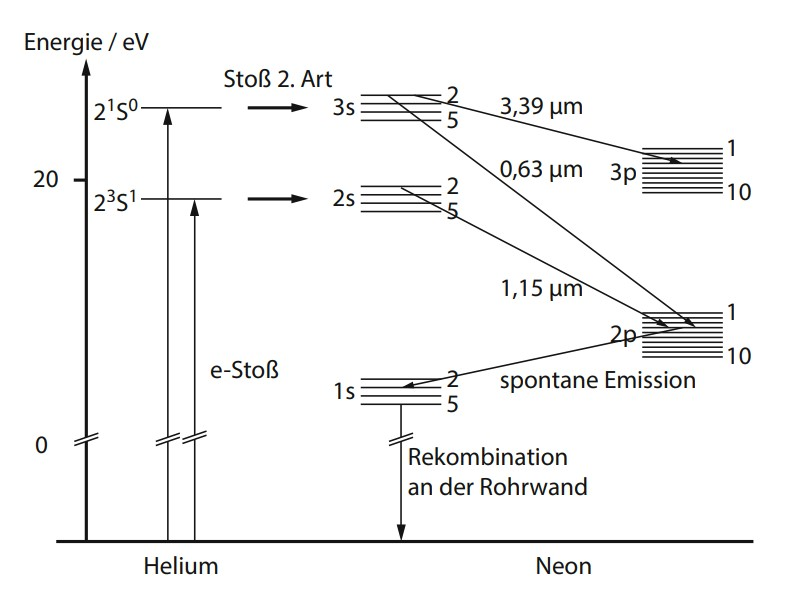
\includegraphics[width=0.6\textwidth]{grafiken/energieniveaus.jpg}
    \caption{Energieterme des Heliums und Neons.\cite{eichler}}
    \label{fig:energieniveaus}
\end{figure}
\noindent Dieser Prozess geschieht entweder spontan oder durch stimulierte Emission. Bei der spontanen Emission wird ein Photon
emittiert, wenn ein Elektron von einem angeregten Zustand in den Grundzustand zurückfällt. Bei der stimulierte Emission wird ein Photon emittiert, wenn ein einfallendes Photon
das Elektron von einem angeregten Zustand in den Grundzustand zurückfallen lässt. Dieses emittierte Photon hat dabei die gleiche Energie, Phase und Ausbreitungsrichtung wie das
einfallende Photon.\\
\subsection{Pumpquelle}\label{sec:pumpquelle}
Das Pumpen ist in diesem Versuch ein elektrischer Entladungsprozess. Dabei wird das Helium durch eine angelegte Spannung ionisiert und in einen angeregten Zustand versetzt.
Durch die Energiepumpe wird im Lasermedium eine vom thermischen Gleichgewicht abweichende Besetzung eines Niveaus erzeugt. Mit ausreichender Pumpenergie kann so eine Besetzungsinversion (angeregter Zustand höhere Besetzungszahl als Grundzustand) erreicht werden.\\
\subsection{Resonator}\label{sec:resonator}
Der Resonator besteht aus zwei Spiegeln, von denen einer teilweise durchlässig ist. Senkrecht auf die Spiegel treffende Photonen verbleiben im Resonator und sorgen für 
eine Verstärkung des Lichts durch stimulierte Emission. Diese Verstärkung ist dabei umso größer, je länger die Verweildauer des Photons im Resonator ist.
Die Verweildauer ist dabei abhängig von der Länge des Resonators und der Reflektivität der Spiegel. Dadurch, dass ein offener Resonator verwendet wird, entsteht gerichtetes Licht, das durch den
teilweise durchlässigen Spiegel austritt.\\
Eine Kennzahl für den Resonator ist der Stabilitätsparameter $g_1 g_2$. Für einen stabilen Resonator gilt 
\begin{equation}
    \label{eqn:stab}
    0 \leq g_1 \cdot g_2 \leq 1
\end{equation}
und ist durch zwei konfokale Spiegel gegeben. Ein konfokaler Spiegel hat den Krümmungsradius $r_1 = r_2 = L/2$, wobei $L$ die Länge des Resonators ist. $g_1$ und $g_2$ ergeben sich mit den
Krümmungsradien und der Resonatorlänge zu
\begin{equation*}
    g_i = 1 - \frac{L}{r_i}.
\end{equation*}
Da die Wellenlänge des Lasers klein gegenüber der Resonatorlänge ist erfüllt nicht nur eine Wellenlänge/Frequenz die Resonanzbedingung, sondern eine ganze Reihe von Moden. Die Transversalmoden
entstehen, da das Licht, das zwischen den Spiegeln reflektiert wird, stehende Wellen ausbildet. 
Grundsätzlich müssen nun einige Bedingungen erfüllt sein, damit ein Laserbetrieb möglich ist. Zum einen muss die Verstärkung größer sein als die Verluste im Resonator. Verluste entstehen
zum Beispiel durch Absorption oder Streuung. Eine Verstärkung (erst unabhängig von Verlusten) ist gegeben, wenn der frequenzabhängige Absorptionskoeffizient $\alpha(\nu)$ negativ ist.\cite{demtroeder}
Für die Intensität entlang der Ausbreitungsrichtung $I(z)$ gilt dann:
\begin{equation*}
    I(z) = I_0 \exp\left(-\alpha(\nu)z\right).
\end{equation*}
Dadurch ergibt sich für die Verstärkung:
\begin{equation*}
    g(\nu) = \frac{I(z)}{I_0} = \exp\left(-\alpha(\nu)z\right).
\end{equation*}
Verluste im Resonator lassen sich mit dem Faktor $\exp(-\gamma)$ beschreiben. Für Hin- und Rückweg im Resonator der Länge $L$ gilt dann für die Verstärkung:
\begin{equation*}
    G = \exp(-2\alpha L - 2\gamma).
\end{equation*}
Die Bedingung für Laserbetrieb ist dann:
\begin{equation*}
    G > 1.
\end{equation*}
\subsection{Mehrniveausystem}\label{sec:mehrniveausystem}
Zudem ist zu beachten, dass ein solcher Laser nicht durch ein Zweizustandssystem beschrieben werden kann, sondern durch ein Mehrniveau-System. In einem Zweizustandssystem würden die Elektronen
nach der Emission eines Photons in den Grundzustand zurückfallen. Dies würde jedoch zu einem schnellen Abklingen der Besetzungsinversion führen beziehungsweise diese erst gar nicht entstehen lassen. 
Die Besetzungsinversion ist aber eine notwendige Bedingung für den Laserbetrieb.\\
\subsection{Modenstruktur}\label{sec:modenstruktur}
Bei der Modenstruktur eines Lasers wird zwischen longitudinalen und transversalen Moden unterschieden. Die longitudinalen Moden entstehen durch die stehenden Wellen, die sich zwischen den Spiegeln
ausbilden. Die transversalen Moden sind durch die Form des Resonators und die Reflektivität der Spiegel gegeben.\\
\subsubsection{Longitudinale Moden}\label{sec:longitudinalemoden}
Wenn Licht in den Resonator eintritt, breitet es sich längs der Ausbreitungsrichtung aus und interagiert mit den reflektierenden Oberflächen.
Dies führt zu stehenden Wellen entlang der Achse des Resonators, wobei die konstruktive Interferenz an bestimmten Frequenzen auftritt, die den longitudinalen Moden entsprechen.
\subsubsection{Transversale Moden}\label{sec:transversalemoden}
Beugung an den Rändern des Resonators führt dazu, dass sich die Lichtwellen innerhalb des Resonators ausbreiten und bestimmte Modenformen annehmen.
Die genaue Form und Verteilung der Transversalmoden hängen von der Geometrie des Resonators ab, einschließlich der Größe der Spiegel und des Abstands zwischen ihnen.
Bezeichnet werden diese Moden mit $TEM_{xy}$, wobei $x$ und $y$ die Anzahl der Knoten in $x$- und $y$-Richtung sind. Die $TEM_{00}$-Mode ist die Grundmode, die sich durch eine Gaußverteilung
der Intensität senkrecht zur Ausbreitungsrichtung auszeichnet. Die Intensitätsverteilung ist dabei gegeben durch
\begin{equation*}
    I(r) = I_0 \exp\left(-2\frac{r^2}{w^2}\right).
\end{equation*}
Höhere Moden ergeben sich mit den Hermite-Polynomen und der Gaußfunktion. Die Intensitätsverteilung der $TEM_{10}$-Mode ist beispielsweise gegeben durch
\begin{equation*}
    I(r) = I_0 \left(\frac{r}{w}\right)^2 \exp\left(-2\frac{r^2}{w^2}\right).
\end{equation*}
Einige Moden sind in \autoref{fig:moden} dargestellt.
\begin{figure}[H]
    \centering
    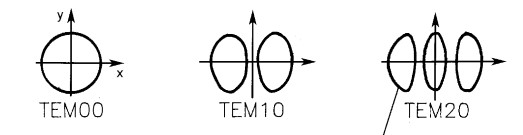
\includegraphics[width=0.6\textwidth]{grafiken/tem.jpg}
    \caption{Intensitätsverteilung der $TEM_{00}$-, $TEM_{10}$- und $TEM_{20}$-Mode.\cite{eichler}}
    \label{fig:moden}
\end{figure}
\subsection{Polarisation}\label{sec:polarisation}
Zur Polarisation des Lichts gibt es verschiedene Möglichkeiten. In diesem Versuch werden Brewster-Fenster am Resonator verwendet, um eine Polarisation des Lichts zu erreichen.
In \autoref{fig:polarisation} ist zu sehen, wie ein Polarisator funktioniert. Es wird sich der Brewster-Winkel zunutze gemacht, bei dem der reflektierte Strahl senkrecht zur reflektierenden
Oberfläche polarisiert ist. Durch die Hintereinanderschaltung von mehreren Brewster-Fenstern kann so auch eine parallele Polarisation erreicht werden.
\begin{figure}[H]
    \centering
    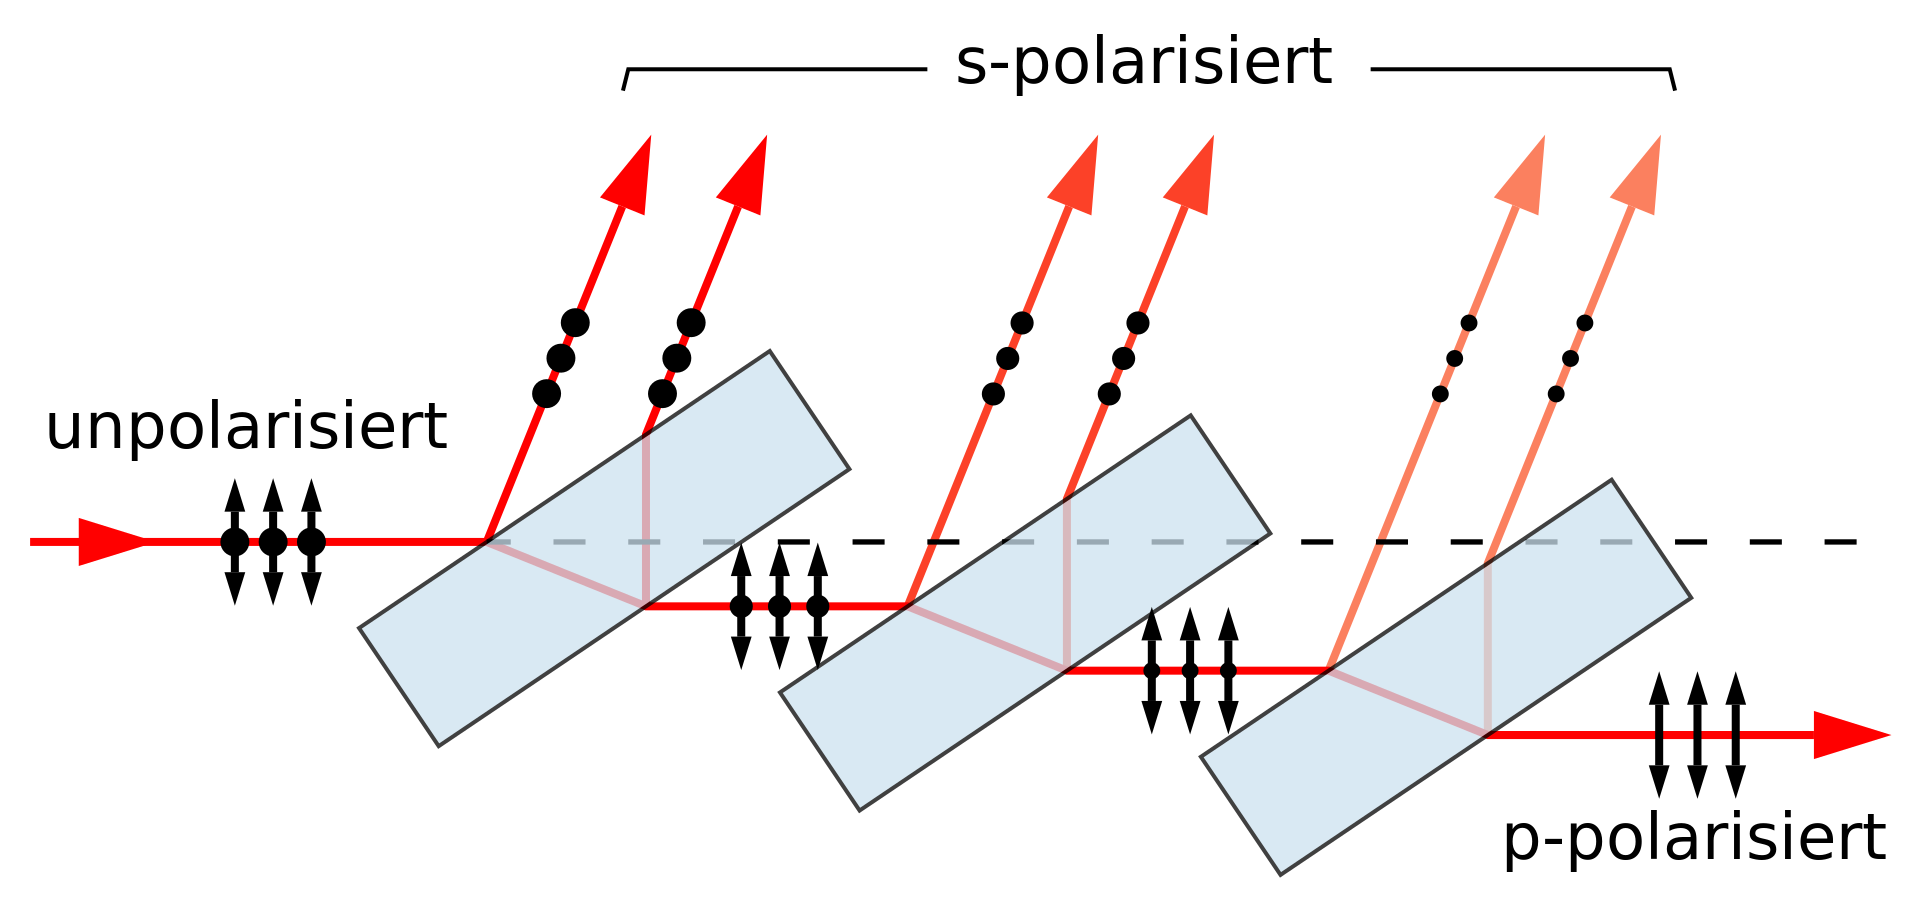
\includegraphics[width=0.6\textwidth]{grafiken/brewster.png}
    \caption{Funktionsweise eines Polarisators.\cite{brewster}}
    \label{fig:polarisation}
\end{figure}
\subsection{Wellenlänge}\label{sec:wellenlaenge}
Die Wellenlänge des Lasers kann durch Beugung an einem Gitter bestimmt werden. Die Wellenlänge ergibt sich mit
\begin{equation*}
    \label{eqn:wel}
    \lambda = \frac{g \cdot a_k}{k \cdot \sqrt{e^2 + a_k^2}},
\end{equation*}
wobei $g$ die Gitterkonstante, $a_k$ der Abstand des $k$-ten Maximums zum Hauptmaximum und $e$ der Abstand des Schirms zum Gitter ist.\\
\newpage
